\documentclass[a4paper,11pt]{article}
\usepackage[left=2cm,text={17cm, 24cm},top=3cm]{geometry}
\usepackage[utf8]{inputenc}
\usepackage[czech]{babel}
\usepackage{times}
\usepackage[hidelinks]{hyperref}
\usepackage{graphicx}
\usepackage{booktabs}
\usepackage{epstopdf}
\usepackage{fancyvrb}
\usepackage{float}
\fvset{frame=single,framesep=1mm,fontfamily=courier,fontsize=\scriptsize,numbers=left,framerule=.3mm,numbersep=1mm,commandchars=\\\{\}}
\usepackage[usenames,dvipsnames]{xcolor}
\graphicspath{{./images/}}
\usepackage{listings}
\lstdefinestyle{customc}{
	abovecaptionskip=0\baselineskip,
	breaklines=true,
	frame=L,
	xleftmargin=\parindent,
	language=C,
	showstringspaces=false,
	basicstyle=\footnotesize\ttfamily,
	keywordstyle=\bfseries\color{green!40!black},
	commentstyle=\itshape\color{purple!40!black},
	identifierstyle=\color{blue},
	stringstyle=\color{orange},
	captionpos=b
}
\renewcommand{\lstlistingname}{Kód}
\lstset{escapechar=@,style=customc}

\begin{document}
\begin{center}
\Huge
\textsc{Vysoké učení technické v~Brně\\
}Fakulta informačních technologií\\
\vspace{\stretch{0.382}}
\LARGE Implementace interpretu imperativního jazyka IFJ16 \\
\Huge Tým 021, varianta a/3/I\\
\vspace{\stretch{0.309}}

\Large Vedoucí:	Kyzlink Jiří 	(xkyzli02)\\
				Kubiš Juraj		(xkubis15)\\
				Korček Juraj	(xkorce01)\\
				Kubica Jan		(xkubic39)\\
				Kovařík Viktor	(xkovar77)\\

\vspace{\stretch{0.309}}

\end{center}
{\Large \today \hfill
Brno}
\thispagestyle{empty}

\newpage

\tableofcontents

\newpage
\section{Úvod}
V této dokumentaci naleznete popis návrhu a implementace interpretu jazyka IFJ16, který je velmi zjednodušenou podmnožinou jazyka Java SE 8, což je staticky typovaný objektově orientovaný jazyk. Vybrali jsme si variantu varianta a/3/I, kde jsme měli za úkol přidat do interpretu vestavěnou funkci find, která využívala Knuth-Morris-Prattův algoritmus a funkci sort, kterou jsme měli implementovat tak, aby využívala shell sort.

--bude ještě doplněno-

\section{Lexikální analyzátor}
Lexikální analyza je založena na deterministickém konečném automatu(dále jen \textit{KA}), jehož vstupem je zdrojový kód programu. Lexikální analyzátor na základě předem definovaných pravidel rozdělí jednotlivé posloupnosti znaků na lexémy, které jsou poslány syntaktickému analyzátoru ve formě tokenu. V tokenu jsou obsaženy informace o typu rozpoznaného lexému, jeho délce, pozici v zdrojovém kódu a odpovídájícimu řetězci ze zdrojového kódu. Vedlejším úkolem lexikální analýzy je odstraňování bílých znaků, ale i řádkových a blokových komentářů. Lexikální analýza je řízena syntaktickou analýzou, která postupně žadá o tokeny. Naše implementace obsahuje funkci \texttt{peek\_token}, která usnadňuje práci syntaktické analýze, protože umožňuje se podívat o jeden token napřed. Klíčové slova, která jse nemůžou vyskytovat v jménech identifikátorů jsou realizovana jako pole řetezců.

Pokud lexikalní analýza narazí na nerozpoznatelný lexém, tak na chybový výstup vypíše hlášení o chybě a řádku na kterém k ní přišlo.
\newpage
\subsection{Diagram konečného automatu lexikální analýzy}
\textbf{KA hlavní schéma:} % bold
\begin{figure}[H]
\centering
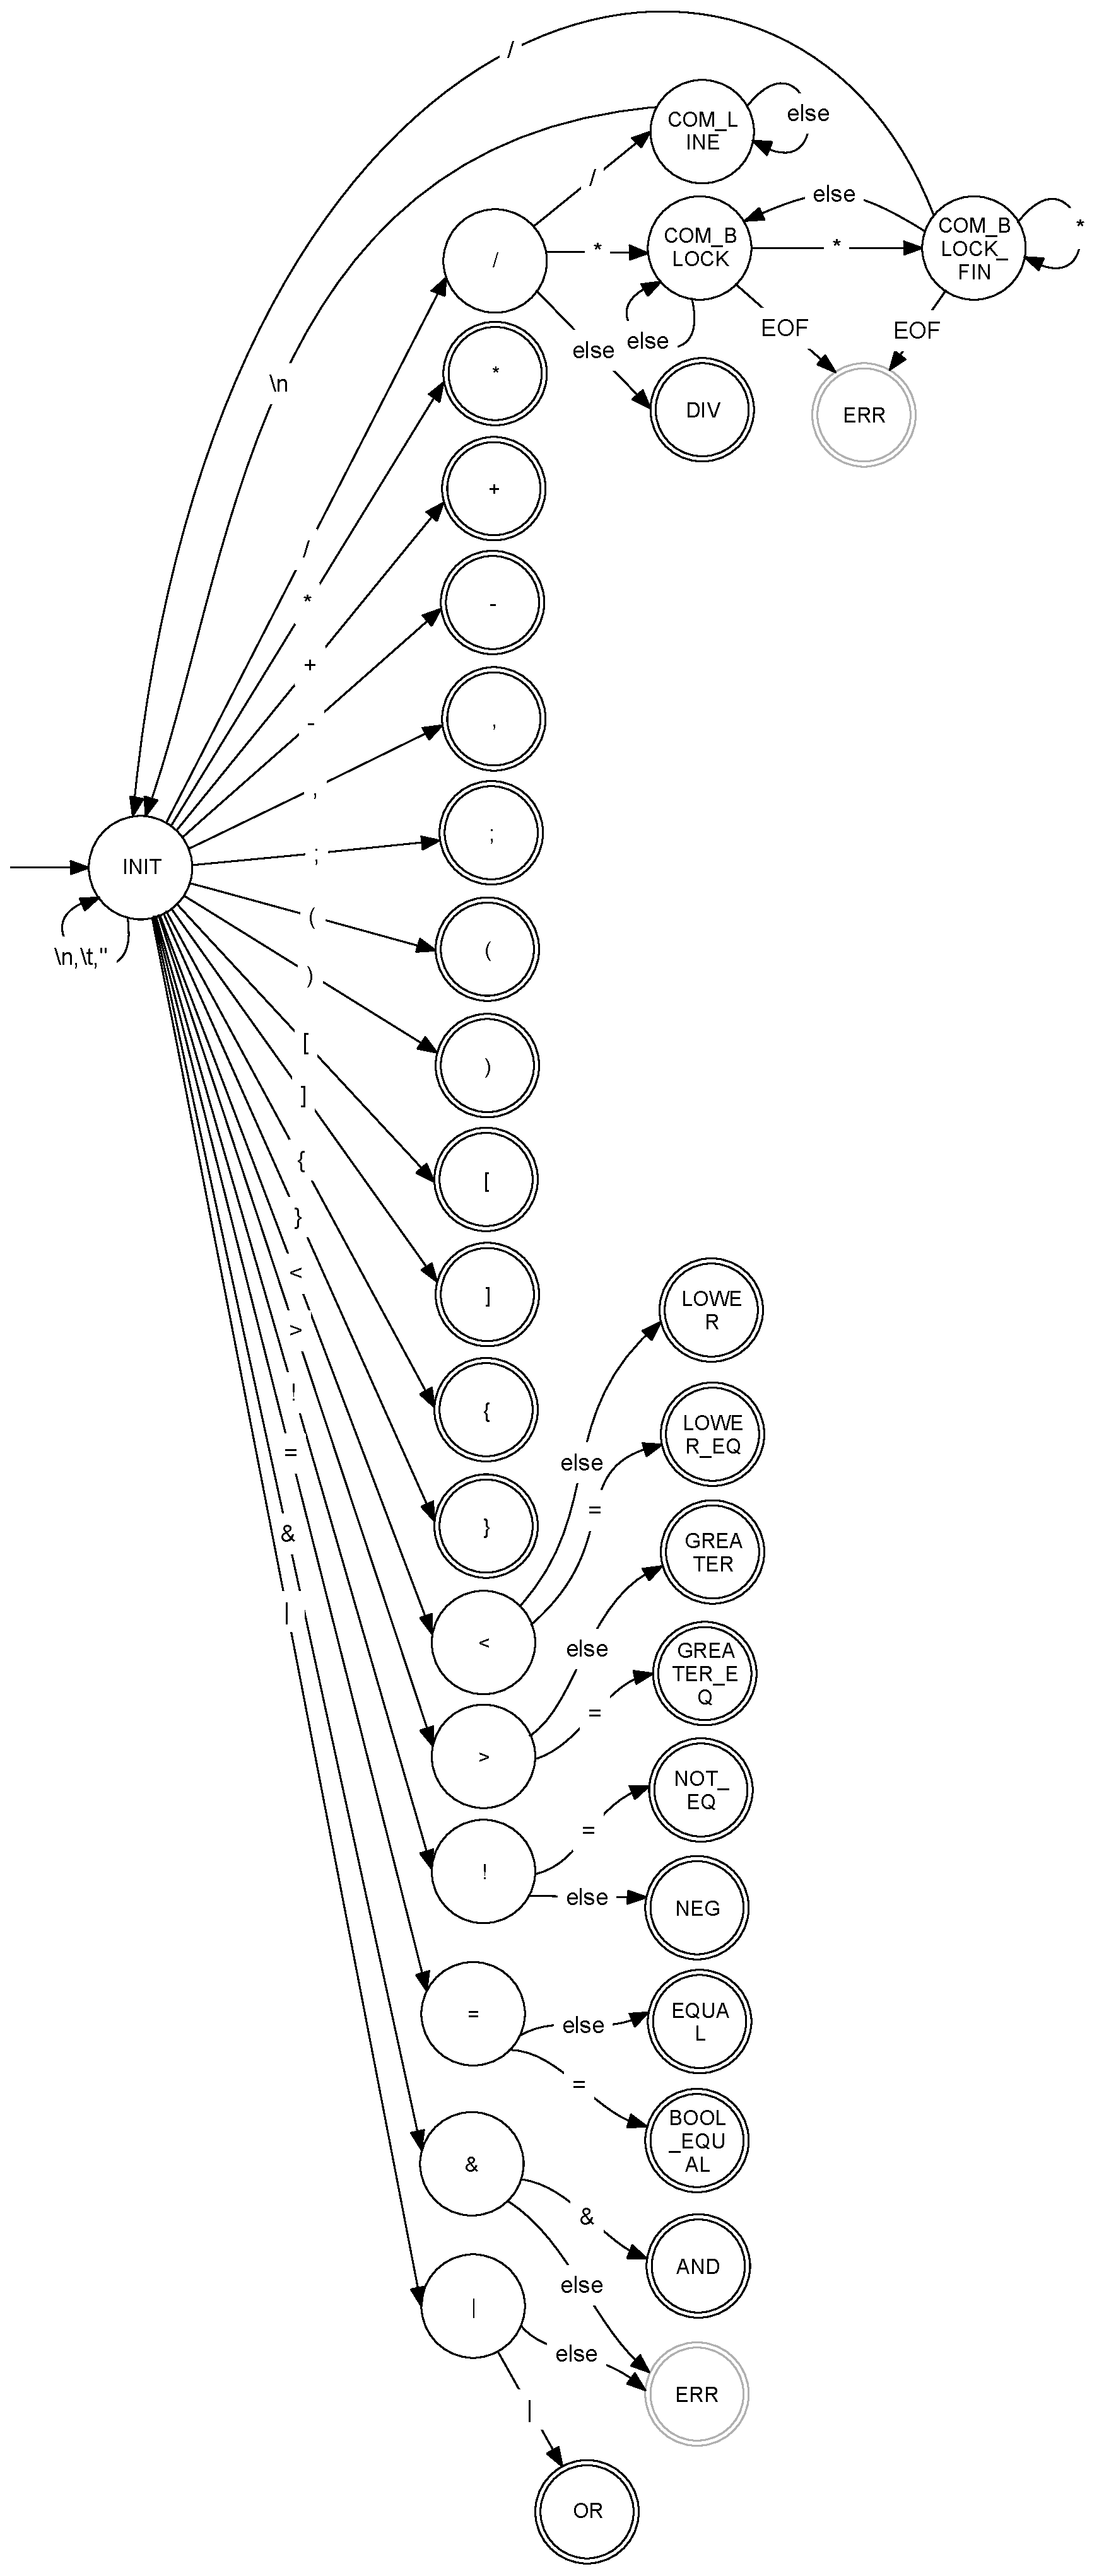
\includegraphics[scale=.31]{FSM_MAIN.eps}
\caption{KA hlavní schéma}
\end{figure}

\newpage
\textbf{KA chyba:} % bold
\begin{figure}[H]
\centering
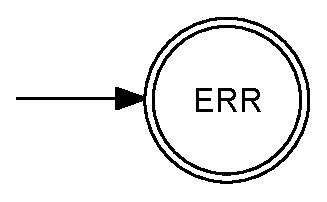
\includegraphics[scale=.31]{FSM_ERR.eps}
\caption{KA chyba}
\end{figure}

\textbf{KA číslicový literál:} % bold
\begin{figure}[H]
\centering
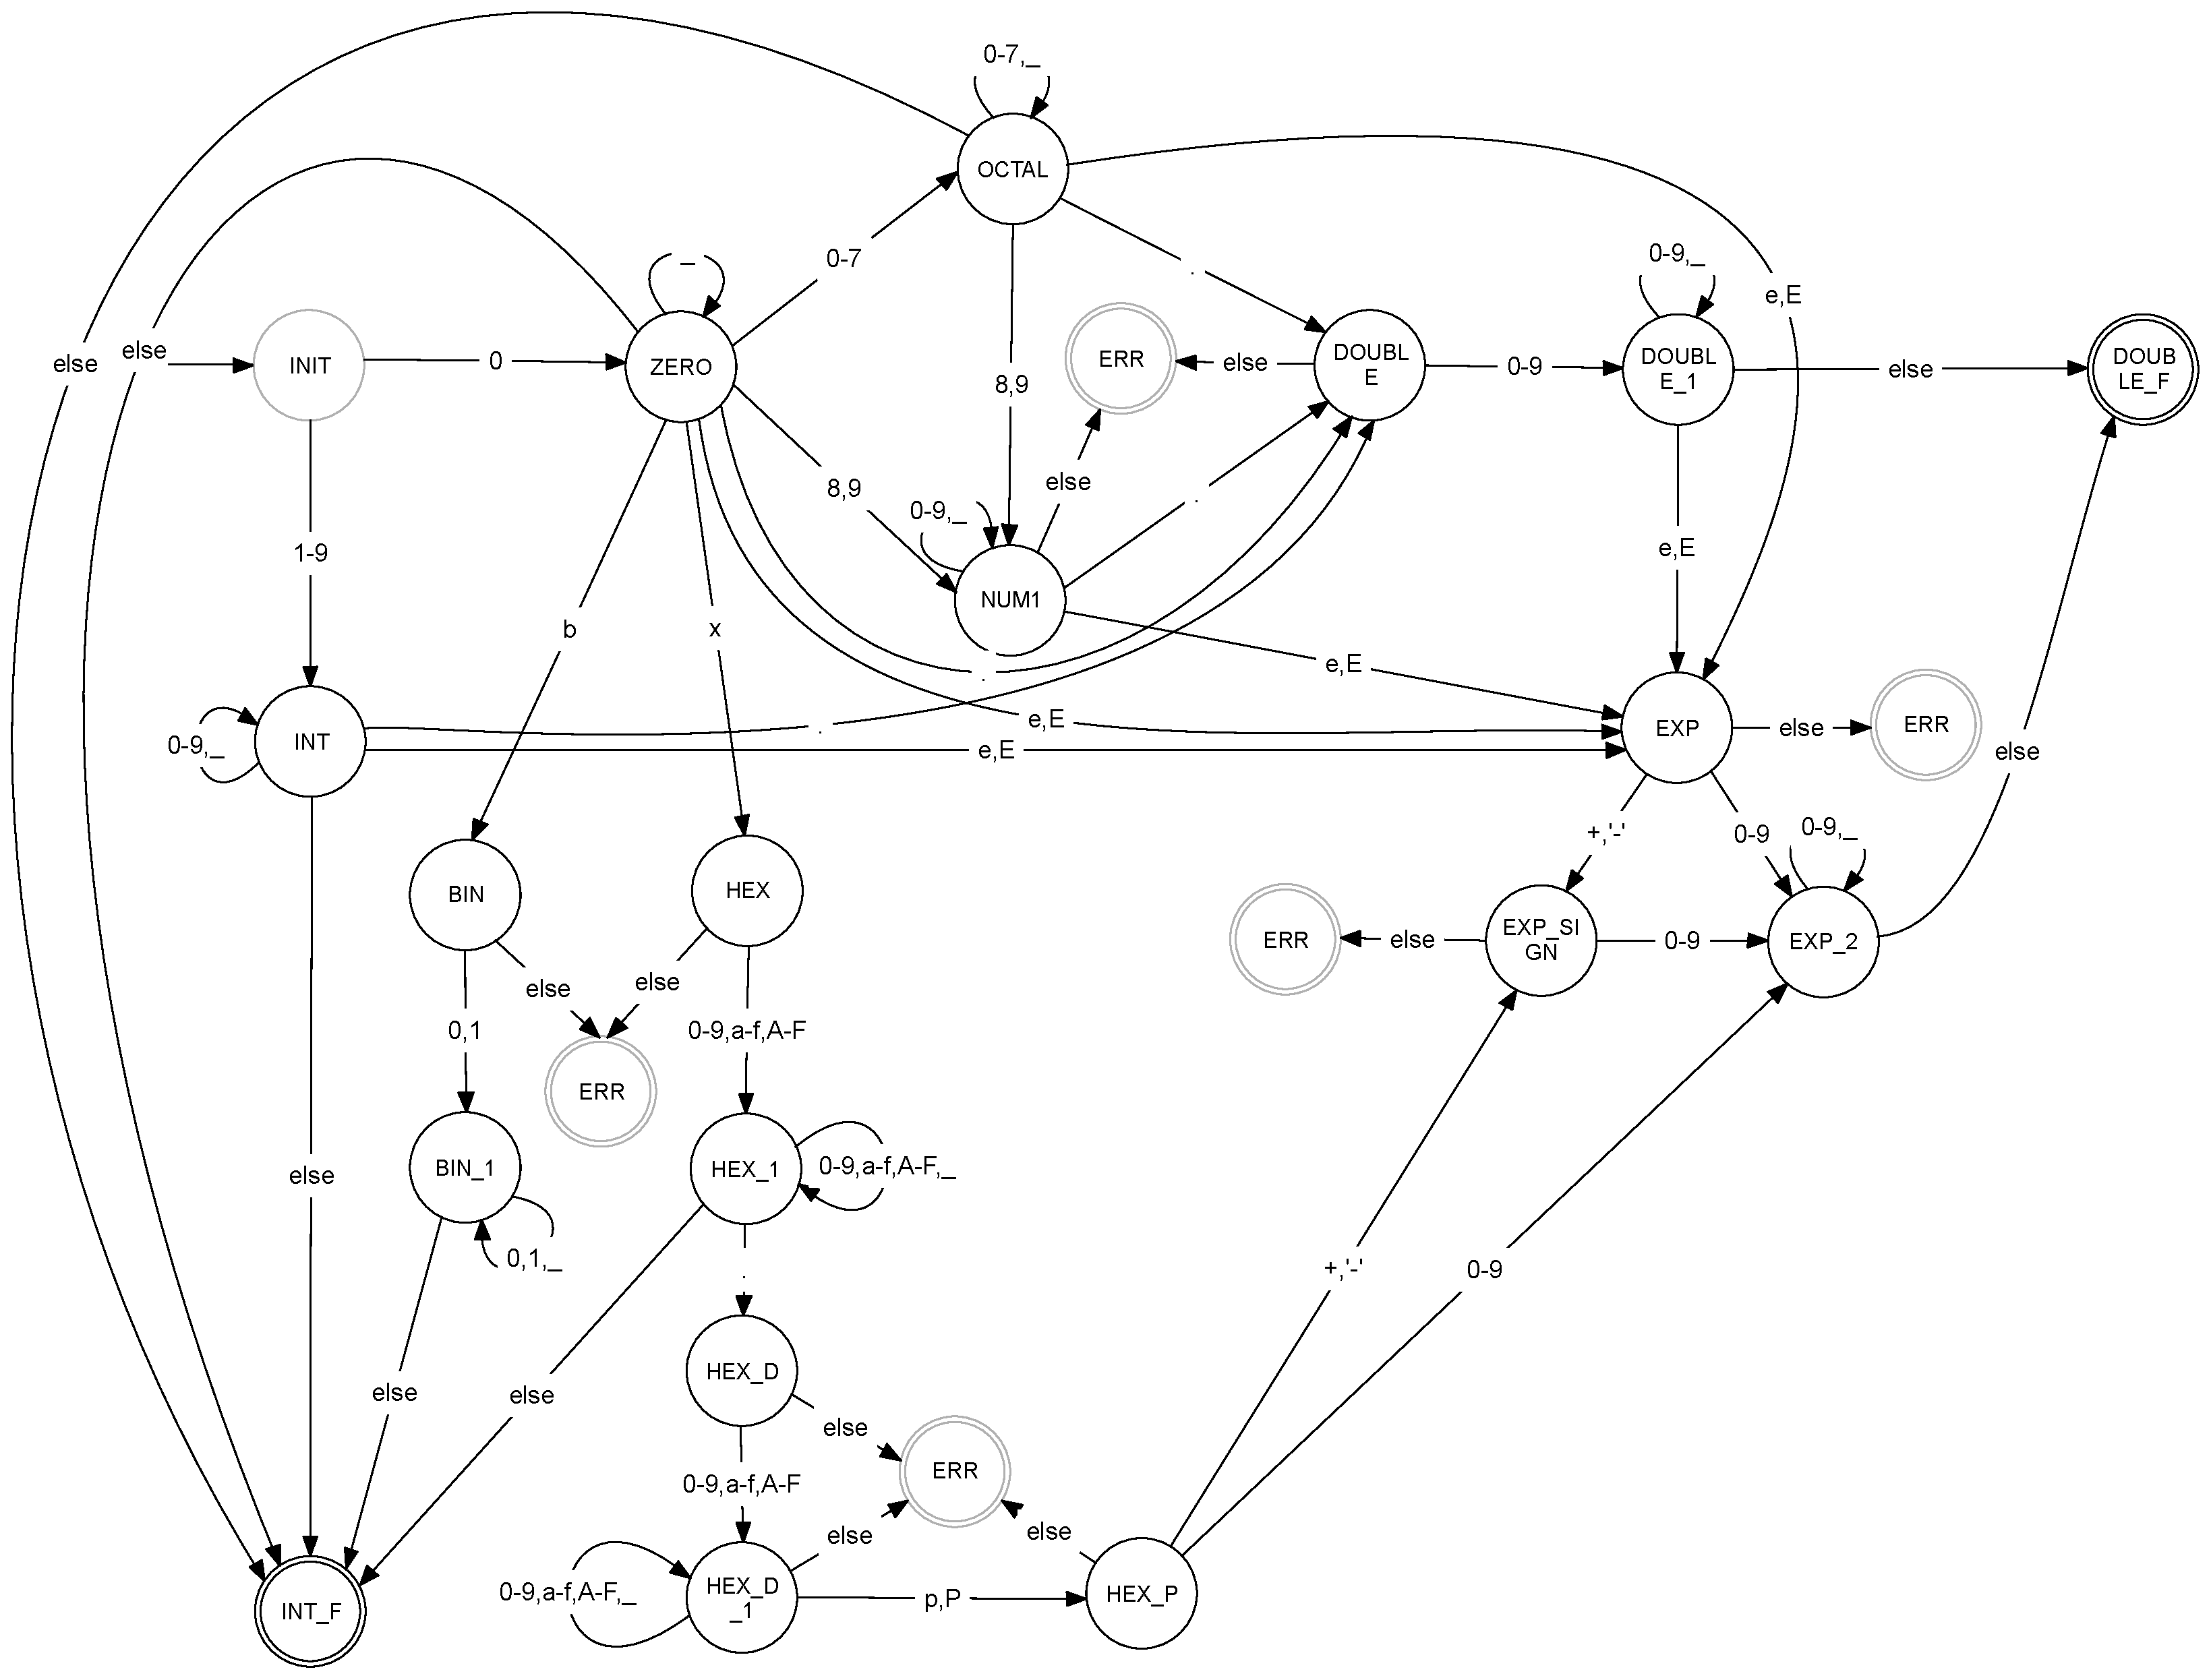
\includegraphics[scale=.31]{FSM_NUM.eps}
\caption{KA číslicový literál}
\end{figure}


\textbf{KA identifikátor:} % bold
\begin{figure}[H]
\centering
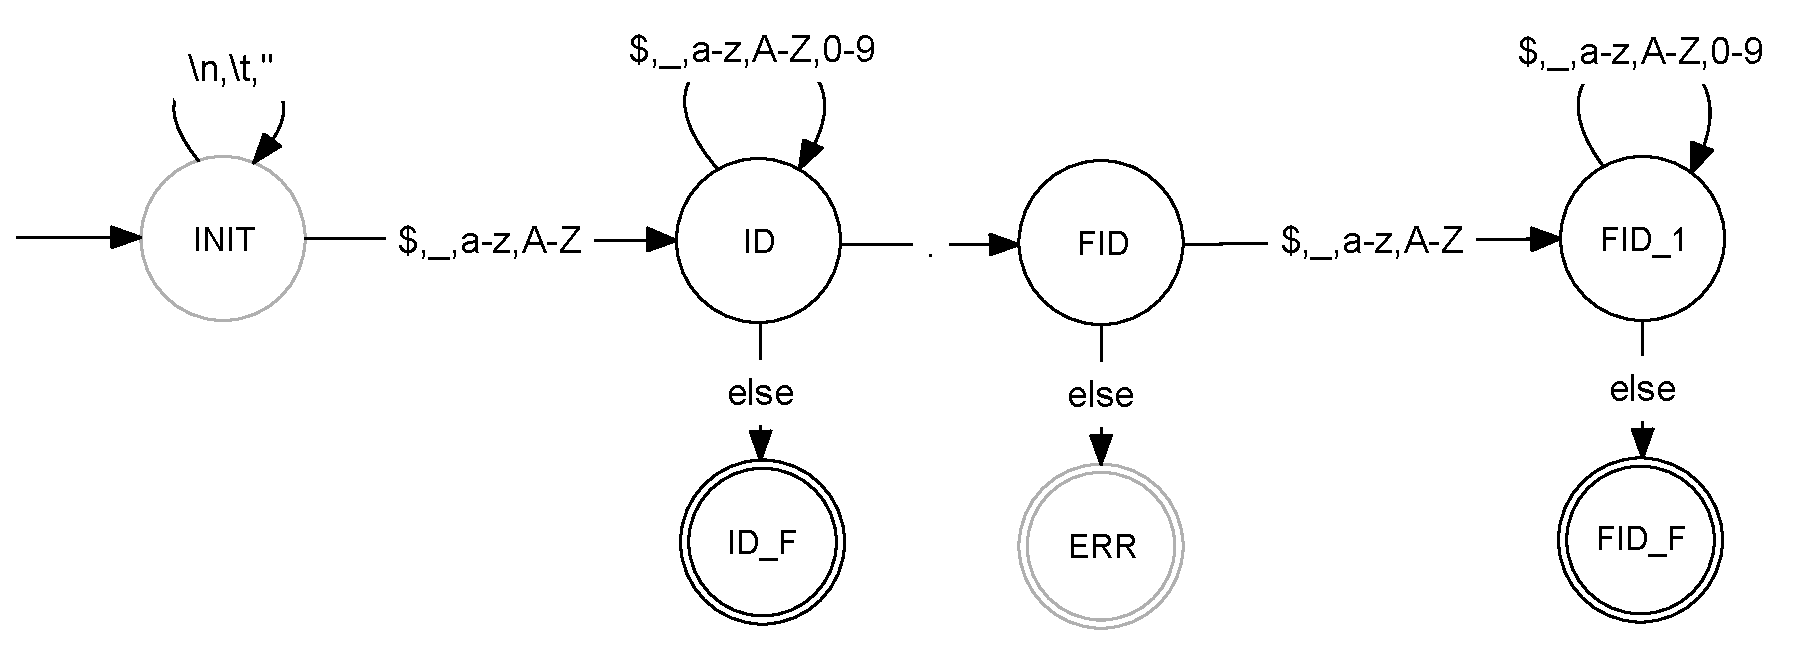
\includegraphics[scale=.31]{FSM_ID.eps}
\caption{KA identifikátor}
\end{figure}

\newpage
\textbf{KA řetězec:} % bold
\begin{figure}[H]
\centering
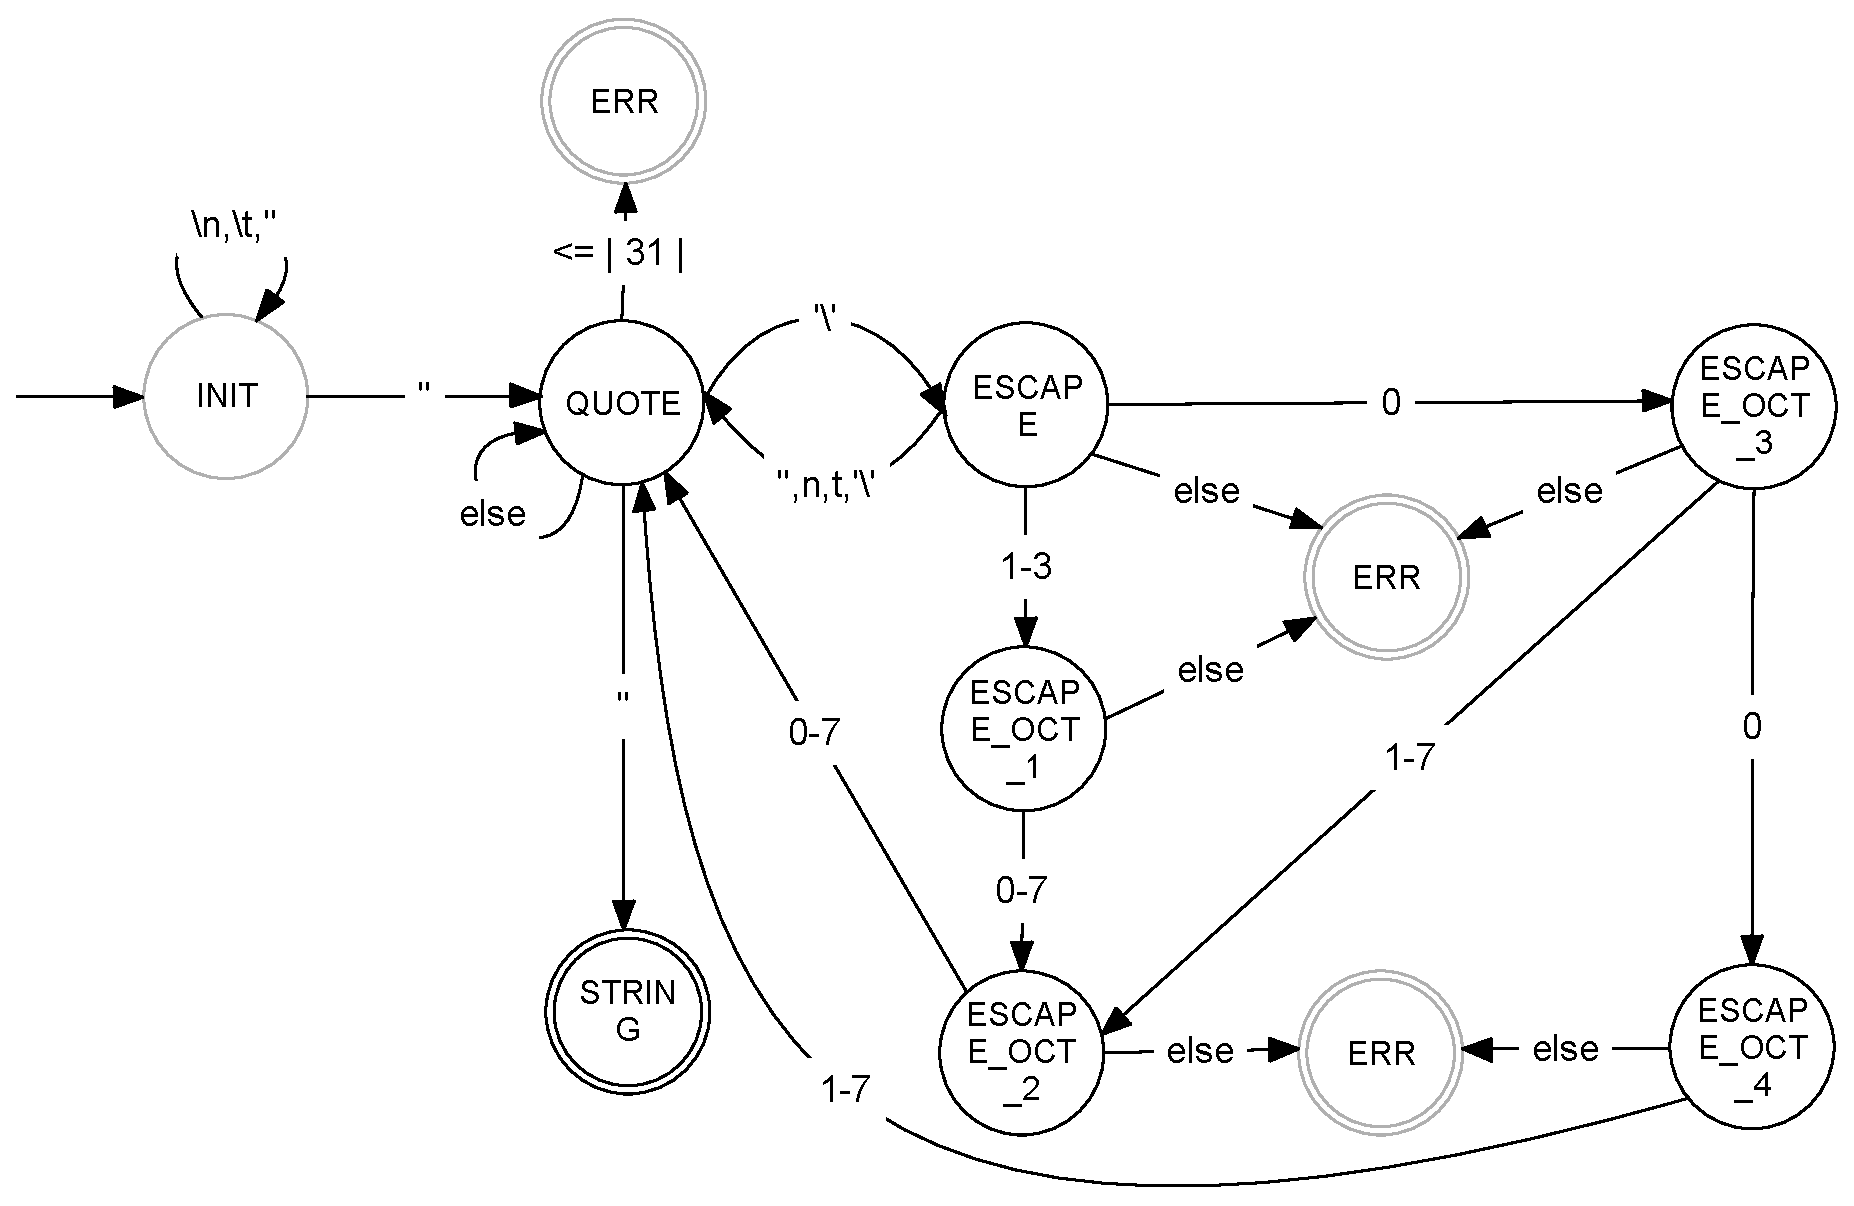
\includegraphics[scale=.31]{FSM_STRING.eps}
\caption{KA řetězec}
\end{figure}



\section{Syntaktický analyzátor}
Syntaktický analyzátor (dále jen \textit{SA}) slouží k vyhodnocování správnosti syntaxe a v našem případě i ke generování abstraktního syntaktického stromu (dále jen \textit{AST}). Vstupen SA je proud tokenů z LA, výstupem je \hyperref[lst:saOut]{struktura} na listingu níže. Struktura obsahuje tybulku globálních symbolů, pro případ kontroly typů, seznam definovaných funkcí, kde každá obsahuje vlastní AST a v posledním prvku je uložen počet globální proměnných pro potřeby alokace paměti.

\begin{lstlisting}[caption={Výstupní struktura SA}, label={lst:saOut}]
typedef struct {
	Symbo_tree global_symbols;
	Function_list functions;
	int globals;
} Syntax_context;
\end{lstlisting}

\subsection{Syntaktická analýza kódu}
Syntaktická analýza kódu je implementovaná pomocí rekurzivního sestupu

\subsection{Syntaktická analýza výrazů}
Úlohou syntaktichého analyzátoru výrazov je správne transformovať výraz na vstupe do podoby AST. Musí pri tom brať na zreteľ prioritu jedtnotlivých operátorov a ich asociativitu.

Zakladom celého analyzátoru je množina pravidiel, precedenčná tabuľka operátorov (ďalej len \textit{tabuľka}) a zásobník. Analýza prebieha spôsobom, že sa prečíta neterminál (token) na vstupe a v tubuľke sa vyhľadá jeho vzťah k neterminálu, ktorý je najbližie vrcholu zásobníka. Tento vzťah určuje, aká akcia je na zásobníku vykonaná (jednotlivé akcie budú vysvetlené nižšie). Následne je prečítaný ďaľší token a celý postup sa opakuje do doby, kedy token na vstupe signalizuje koniec výrazu a na zásobnníku sa nenachádza žiadny neterminál.

\subsubsection{Precedenčná tabuľka operátorov}

Tabuľka vyjadruje vztah medzi každou dvojicou operátorov a určuje aká akcia je na zásobníku vykonaná. Tieto akcie sú:

\begin{table}[]
\centering
%\caption{My caption}
\label{my-label}
\begin{tabular}{@{}ccc@{}}
\toprule
Symbol       & Význam                            & Sématická akcia                         \\ \midrule
=            & Push                              & Token na vstupe je vložený na zásobník  \\
\textless    &                                   & Token na vstupe je vložený na zasobník, \\
\textgreater & Handle                            & Redukcia                                \\
F            & Function call                     & bla                                     \\ \bottomrule
\end{tabular}
\end{table}

\section{Sémantický analyzátor}


\section{Interpret}

\section{Vestavěné funkce}
Vestavěné funkce jsou pro přehlednost rozděleny na dvě části, neboť podle zadání musí být funkce \texttt{find} a \texttt{sort} uloženy právě v souboru \texttt{ial.c}. Ostatní funkce jsou k nalezení v souboru \texttt{build\_in.c}.

\subsection {vestavěné funkce v IAL.c}
--nevím jestli rozdělovat na podsekce ještě měnší nebo ne--

\subsubsection {\texttt{int find(String s, String search)}}
Funkce \texttt{int find(String s, String search)} hledá první výskyt zadaného podřetězce (v parametru \texttt{search}) a vrátí jeho pozici (počítanou od nuly). V naší variantě a/3/I jsme měli za úkol implementovat tuto funkci pomocí \texttt{Knuth-Morris-Prattova algorytmu}. Tato implementace spočívala v ... doplním.

\subsubsection {\texttt{String sort(String s)}}
Funkce \texttt{String sort(String s)} řadí parametrem daný řetězec \texttt{s} podle ordinální hodnoty obsažených znaků, který pak odevzdává návratovou hodnotou. Daný výpočet je dle zadání a/3/I zpracován pomocí řadícího algoritmu \texttt{Shell sort}, nebo též řazení se snižujícím se přírůstkem s asymptotickou složitostí $O(n^{2})$. Styl implementace vychází ze vzorového příkladu přednášek předmětu IAL, kdy při prvním průchodu je brán krok jakožto polovina počtu prvků z celkové délky řetězce.

\subsection {vestavěné funkce v souboru build{\_}in.c}
Pro usnadnění práce při interpretaci jsou zde u funkcí návratové typy zjednodušeny na datový typ \texttt{Value} a parametry funkcí jsou předávány pomocí datového typu \texttt{Value\_list}.

\begin{itemize}
\item {\texttt{int readInt ()}} - funkce zpracovává čtený řetězec ze standardního vstupu po znacích a je zde tak zřejmá podobnost s konečnými automaty. Při nepovoleném znaku pro datový typ \texttt{int} volá funkce ke konci chybové hlášení, jinak je připuštěno k převodu řetězce na celé číslo.
\item {\texttt{double readDouble ()}} - funkce je charakterem obdobná s funkci \texttt{readInt} a výsledná kontrola na desetinné číslo je ošetřena pomocí céčkové funkce \texttt{strtod()}.
\item {\texttt{String readString ()}} - funkce na podobném přístupu jako \texttt{readInt} s rozšířenou množinou povolených znaků.
\item {\texttt{void print ( \emph{term\_nebo\_konkatenace} )}} - funkce tisknoucí svůj vstup na standartní výstup. Zde je ošetřena možnost proměnného počtu parametrů pomocí datového typu \texttt{Value\_list}. 
\item {\texttt{int length(String s)}} - funkce pro zjištění délky daného řetězce, která sama vychází z céčkové funkce \texttt{strlen()}.
\item {\texttt{String substr(String s, int i, int n)}} - funkce tiskne podřetězec daného řetězce \texttt{s} s ošetřením na přesah paměti pomocí céčkové funkce \texttt{strncat()}.
\item {\texttt{int compare(String s1, String s2)}} - funkce porovnává dva dané řetězce na základě céčkové funkce \texttt{strcmp()}.
\end{itemize}

\section{Testy}
Testovali jsme buď součásti - \textit{unit testy}, kde jsme zkoušeli, zda daná funkce správně reaguje na vstupy. Unit testy si dělal každý sám a podle potřeby. Bylo zvykem v Makefile pro unit test udělat zvláštní target, kde se kromě samotné kompilace ještě prováděl \textit{valgrind} test pro ověření možných \textit{memory leaků}. 

Dále jsme dělali ještě systémové testy. To byly vlastně testy samotného interpretu a porovnávání jeho výstupu s výstupem Javy SE 8 s přidanou kompatibilitou s jazykem IFJ16. Test byl vytvořen jako samostatný bash script, který se volal z Makefile. Ve složce test/input/ byly různé programy v jazyce IFJ16 ve formátu \textit{návratovýKód\_názevProgramu.ifj16} s možností přidání ještě souboru se stejným formátem, ale koncovkou .in, kde byla možnost dát vstup na \textit{stdin}. Daný skript pak prošel složku, zjistil, zda jsou v ní obsaženy i soubory typu .in pro právě interpretovaný kód. Pokud byla předpokládaná návratová hodnota 0 (chyby IFJ16 interpretu nemělo smysl překládat v Javě a porovnávat), došlo k interpretaci kódu v Javě i ifj16 interpretu s následným porovnání návratových kódů a výstupů. Vše se zapisovalo do logu, který se nacházel ve stejné složce \textit{input} jako interpretovaný kód. Obrázek níže zobrazuje výsledky testování v průběhu raných fází interpretu.\\


%\begin{figure}
%	\centering
%	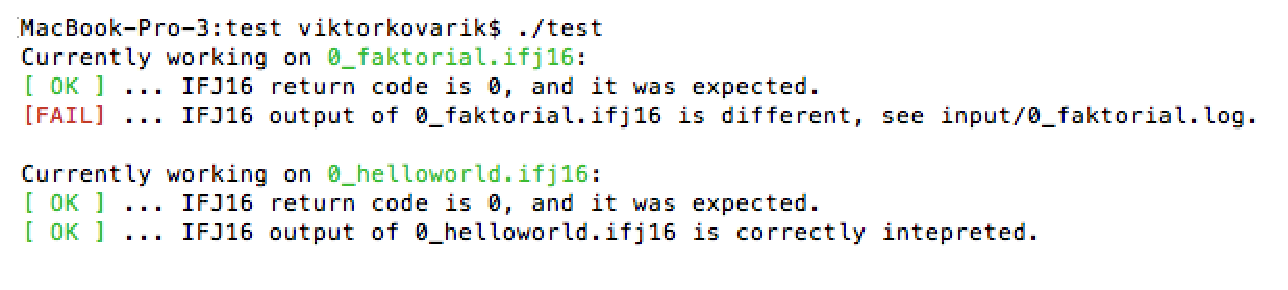
\includegraphics[width=0.7\linewidth]{testy-interpretu.eps}
%	\caption{}
%	\label{fig:testy-interpretu}
%\end{figure}

\begin{Verbatim}
ciUser@travis: ./test
Currently working on 0_ahojsvete.ifj16:
\textbf{\color{green}[ OK ]} ... IFJ16 return code is 0, and it was expected.
\textbf{\color{green}[ OK ]} ... IFJ16 output of 0_ahojsvete.ifj16 is correctly intepreted.

Currently working on 0_arithmetic_test_9_UNARY.ifj16:
\textbf{\color{red}[FAIL]} ... IFJ16 return code is 2, but 0 was expected, see logs/0_fooTest.log.
\textbf{\color{red}[FAIL]} ... IFJ16 output of 0_fooTest.ifj16 is different, see logs/0_fooTest.log.
\end{Verbatim}

\end{document}